\documentclass[accentcolor=tud1c, paper=a4, colorback]{tudreport}
\usepackage[ngerman]{babel}
\usepackage[utf8]{inputenc}

\usepackage{amsmath, imakeidx, graphicx, todonotes, hyperref}

%opening
\title{Bedienungsanleitung Flugsimulator}
\subtitle{BP-Team 19}
\subsubtitle{Wintersemester 17/18}

\newcommand{\ind}[1]{#1\index{#1}}
\graphicspath{ {img/} }

\begin{document}
	\maketitle
	\tableofcontents
	\chapter{Präambel}
	\todo[inline]{basic Infos einfügen}
	\chapter{Einführung}
	\section{Aufbau der Software}
	Aufgrund der Netzwerktopologie ist die Software nach dem sogenannten
	\ind{Client-Server-System}\footnote{\url{https://en.wikipedia.org/wiki/Client-server\_model}}
	aufgebaut.
	\begin{figure}[h]
		\centering
		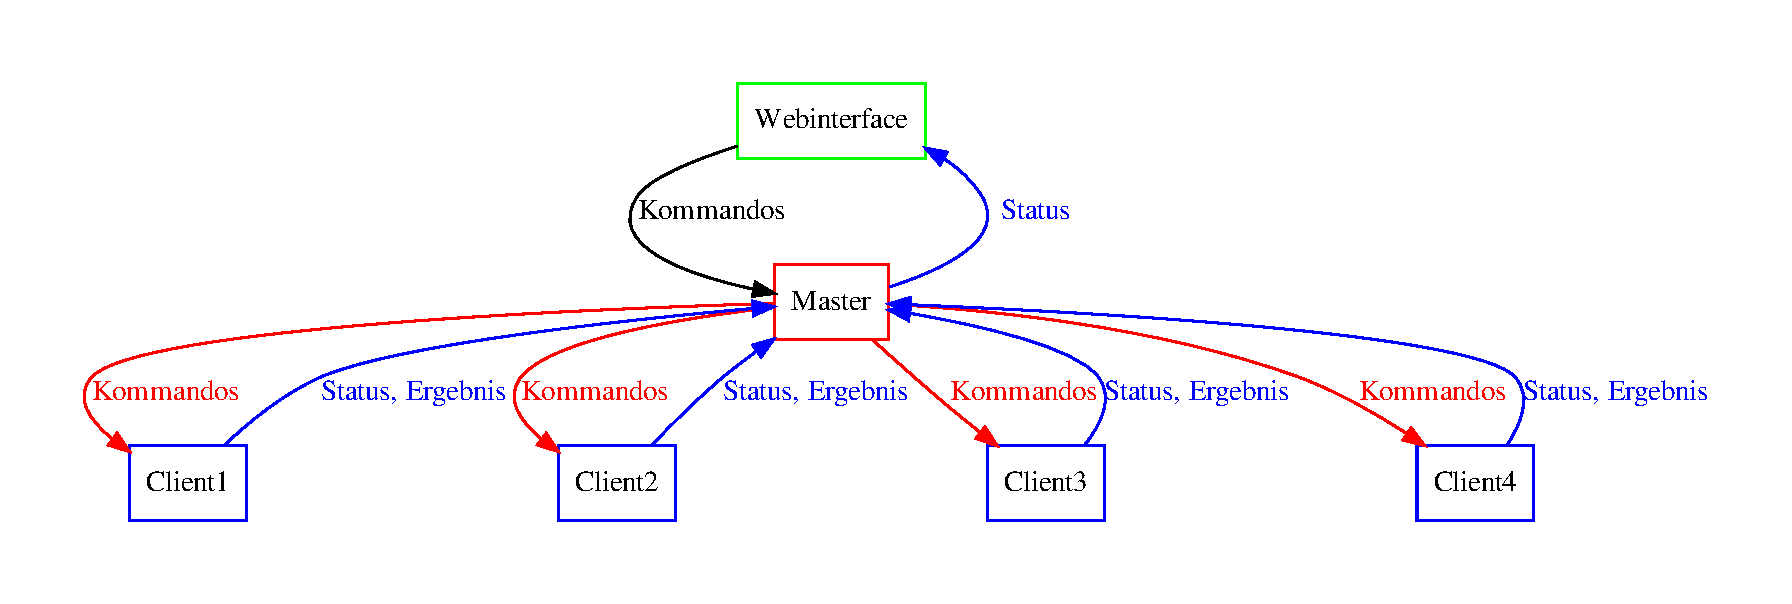
\includegraphics[width=\textwidth]{softwarelayout}
		\caption{Aufbau der Flugsimulatorsteuerung}
	\end{figure}
	\\
	Die Nutzer*innen kommunizieren über ein Webinterface mit dem Masterserver,
	welcher die Befehle dann an die einzelnen Clients weiterleitet.
	\\
	Die Serverkomponente ist in der Programmiersprache \ind{Python}\footnote{\url{https://www.python.org/}}
	in der aktuellen Version 3 geschrieben. Um die Menge an notwendigem Code möglichst
	klein zu halten, wurde auf möglichst verbreitete Frameworks zurückgegriffen.
	Beispielsweise wird das Webinterface auf Serverseite durch das Framework \ind{Django}\footnote{\url{https://www.djangoproject.com/}}
	realisiert, welches sich gerade unter Pythonentwickler*innen sich großer Beliebtheit erfreut.
	Eine Anleitung, wie die Software korrekt aufgesetzt wird, findet sich im Repository des
	Projekts\footnote{\url{https://github.com/bp-flugsimulator/server/blob/master/README.md}}.
	\\
	Die Clients werden ebenfalls von einer Python Software gesteuert. Diese braucht lokal keine Konfiguration,
	bis auf die Adresse des Masterservers. Dieser übernimmt dann die komplette Konfiguration und Steuerung.
	\section{Terminologie}
	Im folgenden werden die einzelnen Begriffe der Software erklärt. Dies dient vor allem dem Verständnis
	der weiteren Kapitel.
	\subsection{Client}
	Ein Client

	\chapter{Workflows}
	\todo[inline]{Standardworkflows a la Eine Node Hinzufügen}



	\todototoc
	\listoftodos

\end{document}
